\section{Model2DRigid\-Dyncar\-Ntire  Class Reference}
\label{class_Model2DRigidDyncarNtire}\index{Model2DRigidDyncarNtire@{Model2DRigid\-Dyncar\-Ntire}}
A 5DOF dynamical model of a rigid car. This model uses a nonlinear tire model. The model was donated by Jim Bernard. 


{\tt \#include $<$model2d.h$>$}

Inheritance diagram for Model2DRigid\-Dyncar\-Ntire::\begin{figure}[H]
\begin{center}
\leavevmode
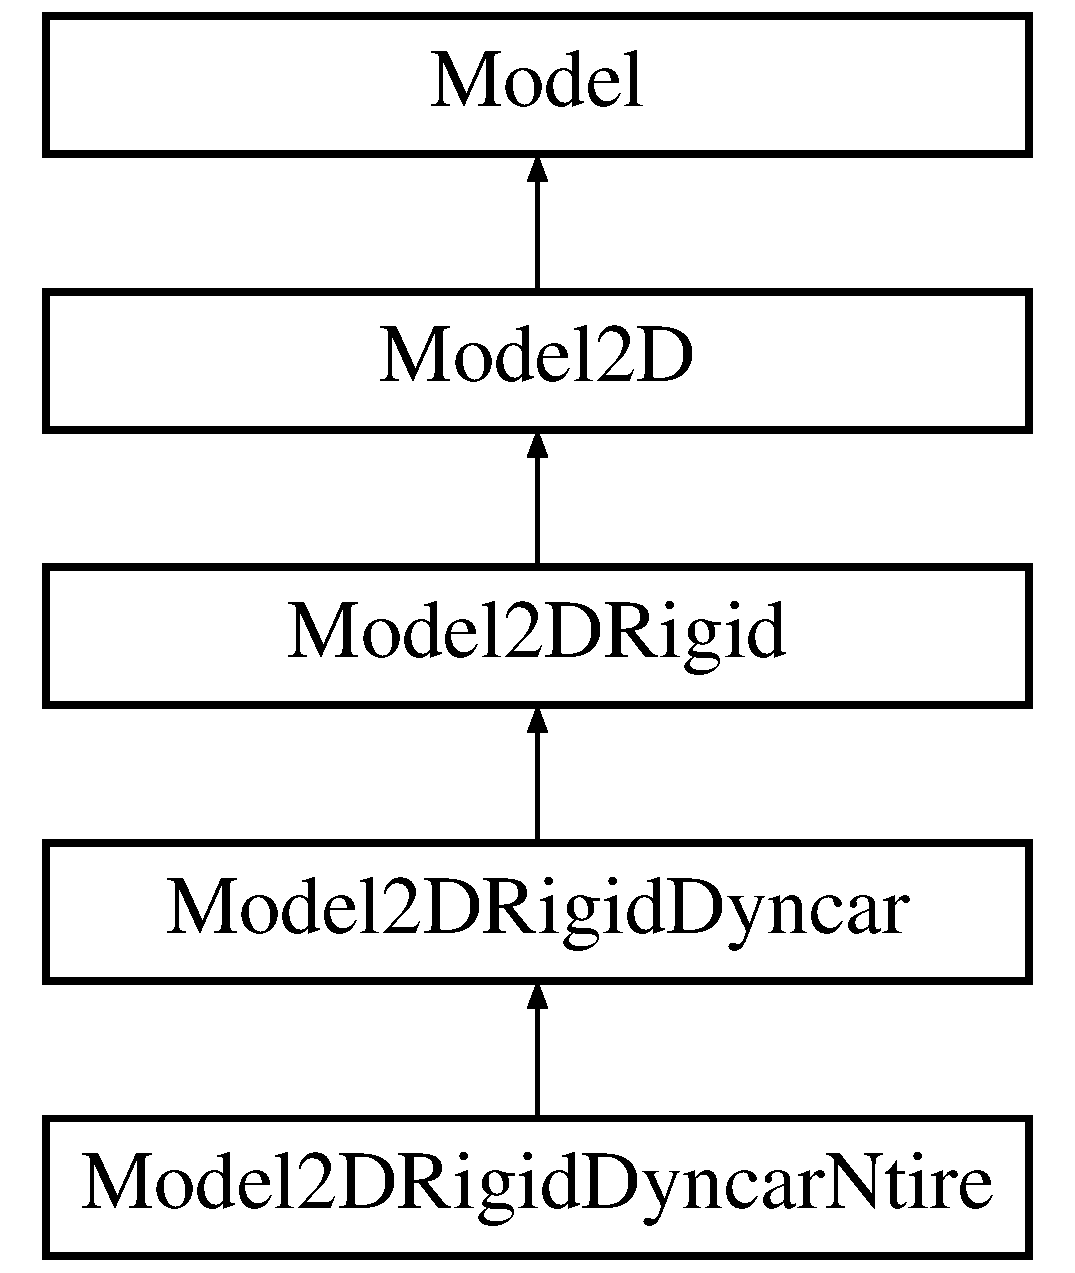
\includegraphics[height=5cm]{class_Model2DRigidDyncarNtire}
\end{center}
\end{figure}
\subsection*{Public Methods}
\begin{CompactItemize}
\item 
{\bf Model2DRigid\-Dyncar\-Ntire} (string path)
\item 
virtual {\bf $\sim$Model2DRigid\-Dyncar\-Ntire} ()
\item 
virtual {\bf MSLVector} {\bf State\-Transition\-Equation} (const {\bf MSLVector} \&x, const {\bf MSLVector} \&u)
\begin{CompactList}\small\item\em The state transition equation, or equations of motion, xdot=f(x,u).\item\end{CompactList}\end{CompactItemize}
\subsection*{Public Attributes}
\begin{CompactItemize}
\item 
double {\bf Mu}
\begin{CompactList}\small\item\em Nonlinear tire model constant.\item\end{CompactList}\item 
double {\bf Nf}
\begin{CompactList}\small\item\em Load on the front tires.\item\end{CompactList}\item 
double {\bf Nr}
\begin{CompactList}\small\item\em Load on the rear tires.\item\end{CompactList}\end{CompactItemize}


\subsection{Detailed Description}
A 5DOF dynamical model of a rigid car. This model uses a nonlinear tire model. The model was donated by Jim Bernard.



\subsection{Constructor \& Destructor Documentation}
\index{Model2DRigidDyncarNtire@{Model2DRigid\-Dyncar\-Ntire}!Model2DRigidDyncarNtire@{Model2DRigidDyncarNtire}}
\index{Model2DRigidDyncarNtire@{Model2DRigidDyncarNtire}!Model2DRigidDyncarNtire@{Model2DRigid\-Dyncar\-Ntire}}
\subsubsection{\setlength{\rightskip}{0pt plus 5cm}Model2DRigid\-Dyncar\-Ntire::Model2DRigid\-Dyncar\-Ntire (string {\em path})}\label{class_Model2DRigidDyncarNtire_a0}


\index{Model2DRigidDyncarNtire@{Model2DRigid\-Dyncar\-Ntire}!~Model2DRigidDyncarNtire@{$\sim$Model2DRigidDyncarNtire}}
\index{~Model2DRigidDyncarNtire@{$\sim$Model2DRigidDyncarNtire}!Model2DRigidDyncarNtire@{Model2DRigid\-Dyncar\-Ntire}}
\subsubsection{\setlength{\rightskip}{0pt plus 5cm}Model2DRigid\-Dyncar\-Ntire::$\sim$Model2DRigid\-Dyncar\-Ntire ()\hspace{0.3cm}{\tt  [inline, virtual]}}\label{class_Model2DRigidDyncarNtire_a1}




\subsection{Member Function Documentation}
\index{Model2DRigidDyncarNtire@{Model2DRigid\-Dyncar\-Ntire}!StateTransitionEquation@{StateTransitionEquation}}
\index{StateTransitionEquation@{StateTransitionEquation}!Model2DRigidDyncarNtire@{Model2DRigid\-Dyncar\-Ntire}}
\subsubsection{\setlength{\rightskip}{0pt plus 5cm}virtual {\bf MSLVector} Model2DRigid\-Dyncar\-Ntire::State\-Transition\-Equation (const {\bf MSLVector} \& {\em x}, const {\bf MSLVector} \& {\em u})\hspace{0.3cm}{\tt  [virtual]}}\label{class_Model2DRigidDyncarNtire_a2}


The state transition equation, or equations of motion, xdot=f(x,u).



Reimplemented from {\bf Model2DRigid\-Dyncar} {\rm (p.\,\pageref{class_Model2DRigidDyncar_a4})}.

\subsection{Member Data Documentation}
\index{Model2DRigidDyncarNtire@{Model2DRigid\-Dyncar\-Ntire}!Mu@{Mu}}
\index{Mu@{Mu}!Model2DRigidDyncarNtire@{Model2DRigid\-Dyncar\-Ntire}}
\subsubsection{\setlength{\rightskip}{0pt plus 5cm}double Model2DRigid\-Dyncar\-Ntire::Mu}\label{class_Model2DRigidDyncarNtire_m0}


Nonlinear tire model constant.

\index{Model2DRigidDyncarNtire@{Model2DRigid\-Dyncar\-Ntire}!Nf@{Nf}}
\index{Nf@{Nf}!Model2DRigidDyncarNtire@{Model2DRigid\-Dyncar\-Ntire}}
\subsubsection{\setlength{\rightskip}{0pt plus 5cm}double Model2DRigid\-Dyncar\-Ntire::Nf}\label{class_Model2DRigidDyncarNtire_m1}


Load on the front tires.

\index{Model2DRigidDyncarNtire@{Model2DRigid\-Dyncar\-Ntire}!Nr@{Nr}}
\index{Nr@{Nr}!Model2DRigidDyncarNtire@{Model2DRigid\-Dyncar\-Ntire}}
\subsubsection{\setlength{\rightskip}{0pt plus 5cm}double Model2DRigid\-Dyncar\-Ntire::Nr}\label{class_Model2DRigidDyncarNtire_m2}


Load on the rear tires.



The documentation for this class was generated from the following file:\begin{CompactItemize}
\item 
{\bf model2d.h}\end{CompactItemize}
